
\documentclass[12pt]{report} 
\usepackage{hyperref} 
\usepackage{amsmath} 
\usepackage{amssymb}
\usepackage{caption} 
\usepackage{float} 
\usepackage{adjustbox} 
\usepackage[margin = 1in]{geometry} 
\pagestyle{myheadings} 
\hypersetup{
	colorlinks 		= true, 
	urlcolor 		= red, 
	linkcolor		= blue, 
	citecolor 		= blue 
}

\begin{document} 
\noindent 
\textbf{Synopsis of Multizone Simulation Results} 
\par\noindent 
\today 
\par\null\par

\begin{center} 
\hypertarget{sec:params}{\textbf{Simulation Parameters}} 
\end{center} 
\par\noindent 
These simulations treat the disk of a Milky Way-like galaxy as a series of 
annular zones with width $\Delta r$ = 250 pc from $R_\text{gal}$ = 0 to 30 kpc. 
These simulations start at time $t$ = 0 with an exponential surface density 
gas disk, which is assumed to be primordial gas: 

\begin{equation} 
\label{eq:sigma_gas} 
\Sigma_g \propto e^{-r/r_\text{s}} 
\end{equation} 
This gas disk is static throughout the simulation; here I'm running VICE in 
\texttt{gas} mode, meaning the mass of the interstellar medium (ISM) is what 
is specified, and I've specified it to be a constant with time for each zone. 
There are inflows and outflows, but with a constant gas mass in each zone, 
VICE is simply solving for the necessary infall rate to balance the mass lost 
to outflows and star formation. Gas is also not migrating between zones in 
this model; there are no radial gas flows. 
\par 
This is running with an implementation of the Kennicutt-Schmidt relation: 
$\dot{M}_\star \propto \Sigma_g^N$, where $N = 1.4 \pm 0.15$ (Kennicutt 1998, 
ApJ, 498, 541). Due to the definition of the star formation efficiency (SFE) 
timescale $\tau_\star \equiv M_g/\dot{M}_\star$: 
\begin{equation}\begin{aligned} 
\dot{M}_\star &\propto \Sigma_g^N \\ 
\implies M_g\tau_\star^{-1} &\propto \Sigma_g^N \\ 
\implies \tau_\star &\propto \Sigma_g^{1 - N} 
\end{aligned}\end{equation} 
With the gas supply given by equation~\ref{eq:sigma_gas}, this mandates a 
scaling of $\tau_\star$ with radius of: 
\begin{equation}
\tau_\star \propto e^{(N - 1)r/r_\text{s}} 
\end{equation}
where $r_\text{s}$ is the scale radius of the gas disk. Beyond 15.5 kpc, I 
have artifically set $\tau_\star = 0$ to shut off star formation and all 
entrainment fractions $\epsilon = 0$. The latter ensures that newly 
synthesized material from stars in a region where star formation is shut off 
is added directly to the outflow as opposed to the ISM. Here I'm showing the 
$\tau_\star(0\text{ kpc})$ = 0.2 Gyr models; even though this model has 
star formation that is likely too vigorous to be realistic, it does the best 
yet at reproducing the observational trends. 
\par 
Prior to the start of VICE's multizone simulation, I assign each star particle 
that will form an ``analog'' from the UW hydro simulation file that Jon Bird 
sent us. To do so, I first set up 40 bins between 0 and 12.8 Gyr (320 Myr width 
time bins), and allow VICE's star particles to find an analog in the hydro 
sim that formed in that time bin and in the same radial bin to the annular 
zone it was born in. If a star does not find an analog here, it is allowed 
to find on in a neighboring zone. If it does not find one in a neighboring 
zone, it stays in the zone it was born in. This ensures that the majority of 
stars in the VICE simulation are radially migrating based on stars that formed 
within approximately one dynamical time (or slightly larger) and at a similar 
radius. 
\par 
\textbf{Only bother reading this paragraph if you want some technical 
justification as to why we don't need to worry about the stars that don't 
find an analog}. 
In the model plotted in this synopsis, VICE formed 317,936 stars. 6743 of 
those stars did not find an analog, 4360 of which formed in the 
$R_\text{gal}$ = 0-250 pc zone. Since we are interested in the disk and not 
the very central region of the galaxy, it's safe to ignore these stars. This 
leaves 2383 star particles which formed in the disk that did not 
find an analog from the hydro simulation - only~$\sim$0.75\% of the star 
particles by number, and~$\sim$1.7\% of the star particles by mass. These 
star particles have a mean (median) formation radius of 2.68 (2.25) kpc with a 
standard deviation of 2.48 kpc, and a mean (median) formation time of 
1.52 (0.18) Gyr with a standard deviation of 3.89 Gyr. Therefore, while these 
``no analog stars'' form somewhat preferentially at early times and small 
radii, they're distributions in $T_\text{form}$ and $R_\text{form}$ are 
sufficiently wide and their contribution to the mass budget sufficiently small 
that they're negligible. 
\par 
This model adopts the following scaling of the mass loading factor 
$\eta = \dot{M}_\text{out}/\dot{M}_\star$ with galactocentric radius: 
\begin{equation} 
\label{eq:eta_r} 
\eta(r) = \frac{y_\text{O}^\text{CC}}{Z_{\text{O},\odot}} 
10^{(0.06\text{ kpc}^{-1})(R_\text{gal} - 4\text{ kpc}) - 0.3} - 0.6 
\end{equation}
This is derived by taking a by-eye linear fit to the mode of the stellar 
[Mg/H] distribution as a function of radius for $0 \leq |z| \leq$ 0.5 kpc 
stars from figure 23 of Weinberg et al. (2018), ApJ, 874, 102 and assuming 
that this corresponds to the equilibrium Mg abundance. This scaling of $\eta$ 
corresponds to $\eta$ = 0.16 at $R_\text{gal}$ = 0 and 1.68 at $R_\text{gal}$ 
= 8 kpc under our yields. This functional form corresponds to the blue line 
in the panel below, while the red line is the linear scaling that we employed 
in some of our first models. 

\begin{figure*}[!h] 
\centering 
\includegraphics[scale = 0.5]{../plots/eta_r.pdf} 
\caption{In blue is the scaling of $\eta$ with galactocentric radius given by 
equation~\ref{eq:eta_r}.}
\end{figure*}

\begin{figure*}[!h] 
\centering 
\includegraphics[scale = 0.3]{../plots/rgal_birth/hayden2015plot/moddisk_vigorousSF.png} 
\caption{Each panel corresponds to a bin in galactocentric radius 
$R_\text{gal}$ (denoted at the top of each column) and height above/below the 
plane $\left|z\right|$ (denoted in the middle panel of each column). Points 
are color-coded according to the $R_\text{gal}$ at which each star was born, 
and their size scales linearly with their mass. There is a bimodality most 
apparent in the $R_\text{gal}$ = 5 - 7 kpc bin, in agreement with 
observations.} 
\end{figure*} 

\begin{figure*}[!h] 
\centering 
\includegraphics[scale = 0.3]{../plots/age/hayden2015plot/moddisk_vigorousSF.png}
\caption{
Same as above, but points are color-coded by age in Gyr. Of particular 
interest is the population of young (age $\lesssim$ 1 Gyr) stars with mild 
$\alpha$-enhancements seen in many of these panels; this suggests that a 
population of young $\alpha$-rich stars is a natural consequence of radial 
migration. 
} 
\end{figure*} 

\begin{figure*}[!h] 
\centering 
\includegraphics[scale = 0.3]{../plots/age-metallicity/moddisk_vigorousSF.png} 
\caption{
The age-metallicity relation as predicted for the solar annulus (7 kpc $\leq$ 
$R_\text{gal} \leq$ 9 kpc). Points are color-coded according to their 
galactocentric radius of birth, and their size scales linearly with their 
mass. Black stars are plotted at the mass-weighted median age of stars in 
0.1-dex width bins in [O/H]. The model predicts an old, metal rich population 
to originate from the inner regions of the disk, and the young $\alpha$-rich 
population to originate from the outer regions of the disk. 
}
\end{figure*}

\begin{figure*}[!h] 
\centering 
\includegraphics[scale = 0.5]{../plots/gradients/stellar_surface_density/moddisk_vigorousSF.png} 
\caption{
The stellar mass surface density defined by 
$\Sigma_\star \equiv M_\star / (\pi(r_\text{out}^2 - r_\text{in}^2))$ as a 
function of galactocentric radius, normalized to an arbitrary constant. While 
this model was ran with a scale radius of the gas disk of $R_\text{s,g}$ = 3 
kpc, the stellar disk has a scale radius of $R_{\text{s,}\star}$ = 2 kpc, and 
is well-described by the exponential. 
}
\end{figure*}

\begin{figure*}[!h] 
\centering 
\includegraphics[scale = 0.4]{../plots/gradients/metallicity/moddisk_vigorousSF.pdf} 
\caption{
The gradients in [O/H] (left; red), [Fe/H] (left; blue), and [O/Fe] (right). 
Stars represent the mode of the stellar metallicity distribution in their zone, 
shaded regions represent the 16th and 84th percentiles thereof, and the lines 
denote the metallicity of the gas in that zone at the final timestep. The 
drop in overall abundance [X/H] and the increase in [O/Fe] at $R_\text{gal}$ = 
15.5 kpc is due to the artificial shut-off of star formation at radii larger 
than this and the entrainment fractions to zero (all nucleosynthetic products 
go directly to the outflow at these radii). 
}
\end{figure*}

\begin{figure*}[!h] 
\centering 
\includegraphics[scale = 0.7]{../plots/Ia_rate/moddisk_vigorousSF.png} 
\caption{
Proxies for the SN Ia rate as a function of cosmic time at 
$R_\text{gal} \approx$ 5 kpc (blue), 10 kpc (green), and 15 kpc (red) compared 
to what is expected in a one-zone model with the same parameters (dashed lines 
of the same colors). All three rates show low-amplitude white noise on top of 
higher-amplitude variability on Gyr timescales which is not sinusoidal, 
introducing scatter in the relationship between age and [Fe/H], and by 
extension [O/Fe]. In the $R_\text{gal}$ = 15 kpc bin, the fractional amplitude 
of the variability is much larger, and the rate overall is considerably lower 
than the corresponding one-zone model prediction for the majority of the 
simulation. This suggests that the migration of star particles out of this 
zone is not balanced by the migration of star particles from other zones, when 
weighted by the SN Ia rate. Stars migrate away from these radii on short 
timescales, while stars migrate toward these radii on long timescales, leaving 
the outskirts of the disk Fe-poor. This suggests that the young $\alpha$-rich 
stars seen in our simulations are not necessarily $\alpha$-rich but Fe-poor. 
}
\end{figure*}


\end{document}
